
\section{\trActionFunctional}
\label{sec:action-functional}

\subsection{\trLoopSpace}
\label{subsec:loop-space}

我们要找的是某一个特定\trVectorField{}的\trPeriodic\trTrajectory，特别是些 $\cC^\infty$ 映射
\[
x\colon\RR/\ZZ\longrightarrow W\text{。}
\]
因此我们将不得不考虑这些映射所成的空间（以代替\trManifold{} $V$）。

\textbf{\trFixedPoint{}所在的\trConnectedComponent。}

当然，全体\trLoop{}所成的空间一般并不\trConnected：两条不\trHomotopic{}的\trLoop{}显然不落在同一个\trConnectedComponent{}之中。于是我们将把自己限制在一个\trConnectedComponent{}里，而自然的做法是选取包含诸常值\trLoop{}的那一个，因为这些常值\trLoop{}恰好对应\trAutonomous{}情形下的\trCriticalPoint。设 $\scr{L}W$ 是\trManifold{} $W$ 上\trContractible{}的\trLoop{}所成的空间，也就是 $\cC^{\infty}$ 映射
\[
x\colon S^1\longrightarrow W
\]
（自由\trLoop\footnote{这意思是说，\trLoop{}的基点并不固定。此外，这些\trLoop{}之间的\trHomotopic{}也是自由的。}）当中与常值映射\trHomotopic{}的那些。

这个空间被赋予 $\cC^\infty$ \trTopology{}以及一个定义此\trTopology{}的距离函数 $d_\infty$（必要时可参见\cref{subsec:ck-topology}）。它是道路\trConnected{}的（我们可以用一条道路把每条\trLoop{}连到常值\trLoop{}上，这条道路就是两者之间的一个\trHomotopic）。

\textbf{\trFundamentalGroup。}

让我们在\trLoopSpace{}中固定一个基点，也就是等于在 $W$ 中选定的一点 $x_0$ 的那条常值\trLoop；这条\trLoop{}我们也将记作 $x_0$。$\scr{L}W$ 中一条以 $x_0$ 为基点的\trLoop{}是一个映射
\[
\begin{aligned}
\gamma\colon[0,1]\times S^1&\longrightarrow W\\
(s,t)&\longmapsto\gamma(s,t)
\end{aligned}
\]
满足
\[
\gamma(0,t)=\gamma(1,t)=x_0(t)=x_0\text{。}
\]
这可以看成是一个映射 $\tilde{\gamma}\colon S^2\to W$（\cref{fig:loop-cylinder-sphere}）。

\begin{figure}[htbp]
\centering
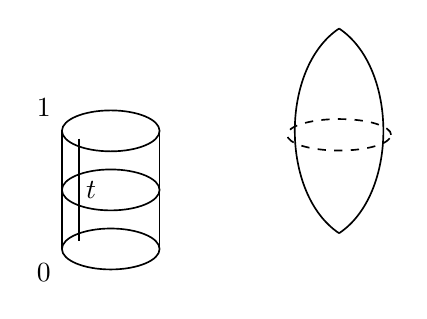
\begin{tikzpicture}[line width=0.6pt]
  \draw (0,0) ellipse (0.62 and 0.26);
  \draw (-0.62,0) -- (-0.62,-1.5);
  \draw (0.62,0) -- (0.62,-1.5);
  \draw (0,-0.75) ellipse (0.62 and 0.26);
  \draw (0,-1.5) ellipse (0.62 and 0.26);
  \draw (-0.4,-0.1) -- (-0.4,-1.4);
  \node at (-0.85,0.3) {$1$};
  \node at (-0.85,-1.8) {$0$};
  \node at (-0.25,-0.75) {$t$};
  \begin{scope}[shift={(2.9,0)}]
    \draw (0,1.3) .. controls (-0.75,0.8) and (-0.75,-0.8) .. (0,-1.3);
    \draw (0,1.3) .. controls (0.75,0.8) and (0.75,-0.8) .. (0,-1.3);
    \draw[dashed] (0,-0.05) ellipse (0.66 and 0.2);
  \end{scope}
\end{tikzpicture}
\caption{}
\label{fig:loop-cylinder-sphere}
\end{figure}

\textbf{\trManifold{}结构、\trTangentSpace。}

把 $\scr{L}W$ 当作一个\trManifold{}来看待是很自然的。起初，我们几乎不需要显式给出这个\trManifold{}结构：它是以一种相当形式化的方式被使用的，方程与论证都在 $W$ 中进行。为了给第 8 章的种种探讨做准备，我们将在本章末尾（\cref{sec:banach-manifold-lw}）描述这个结构。眼下我们唯一需要理解的，是在一点 $x\in\scr{L}W$ 处的切向量是什么。如果把 $x$ 处的一个切向量看成经过 $x$ 的诸曲线的一个等价类，那么我们就需要考虑一条曲线 $s\mapsto u(s)\in\scr{L}W$，$u(0)=x$，此时
\[
\begin{aligned}
\RR\times S^1&\longrightarrow W\\
(s,t)&\longmapsto u(s,t)\qquad\text{其中}\;u(0,t)=x(t)\text{。}
\end{aligned}
\]
于是我们有
\[
\frac{\partial}{\partial s}u(s,t)\big|_{s=0}\in T_{x(t)}W\text{，}
\]
从而很自然地把 $\scr{L}W$ 在 $x$ 处的一个切向量看成沿 $x$ 定义的、切于 $W$ 的一个\trVectorField，也就是说 $x^\star TW$ 的一个\trSection，
\[
Y(t)\in T_{x(t)}W\qquad\text{对一切 }t\in S^1\text{。}
\]
我们也可以把 $Y$ 看成映射
\[
Y\colon\RR\longrightarrow TW\qquad\text{满足 }
\left\{\begin{array}{l}
Y(t)\in T_{x(t)}W\\
Y(t+1)=Y(t)
\end{array}\right.\qquad\forall t\in\RR\text{，}
\]
（另见第~14~章的\cref{ex:ch14-024-loop-space-derivation}。）
一个 $1$-形式 $\alpha$，比如一个函数的\trDifferential，就在 $x$ 处的这些切向量所成的集合上定义了一个线性形式。

\subsection{\trActionFunctional}
\label{subsec:action-functional-b}

这里 $W$ 是一个赋予了\trSymplecticForm{} $\omega$ 的\trManifold，而 $H$ 是一个依赖时间的\trHamiltonian，
\[
\begin{aligned}
W\times\RR&\longrightarrow\RR\\
(x,t)&\longmapsto H_t(x)
\end{aligned}
\]
我们假定它关于 $t$ 是\trPeriodic{}的，也就是说满足
\[
H_{t+1}(x)=H_t(x)\qquad\forall t\in\RR\text{，}
\]
这由注记 6.1.3 所允许。考虑表达式
\[
\scr{A}_H(x)=-\int_D u^\star\omega+\int_0^1H_t(x(t))\,dt\text{，}
\]
其中 $u$ 是 $x\colon S^1\to W$ 到\trDisk{}上的一个扩张，也就是说，是一个映射 $D=\{z\in\CC\mid |z|\le 1\}\to W$，满足 $u(e^{2\pi it})=x(t)$。
第二个积分是\trWellDefined{}的，但\emph{\trApriori}依赖于 $u$ 的选取。若 $v$ 是另一个扩张，则
\[
\int_D u^\star\omega-\int_D v^\star\omega=\int_{S^2}w^\star\omega\text{，}
\]
其中 $w$ 由把两个\trDisk{}沿它们的公共边界\trGluing{}而定义（\cref{fig:disk-gluing-sphere}）。\cref{thm:symplectic-asphericity}意味着\trSymplecticForm{} $\omega$ 的\trRham\trCohomology{}类在 $\pi_2$ 上为零，而正如我们所注意到的，这也可以写成
\[
\langle\omega,\pi_2(W)\rangle=0\text{。}
\]
特别地，若 $\pi_2(W)=0$——也就是说 $\scr{L}W$ 是\trSimplyConnected{}的——则这个条件满足（另见\cref{sec:functions-forms-covers}，本章的一个附录）。\footnote{译注：原书作 “$\pi_2(W)=0$, that is, $\scr{L}W$ is simply connected”，把 $\pi_2(W)=0$ 等同于 $\scr{L}W$ \trSimplyConnected{}；这并不成立：$\pi_2(W)=0$ 推不出 $\scr{L}W$ \trSimplyConnected。事实上，常值\trLoop{}的\trEmbedding{} $c\colon W\to\scr{L}W$（把点 $x$ 对应到点 $x$ 处的常值\trLoop）与求值映射 $\operatorname{ev}_0\colon\scr{L}W\to W$（$\gamma\mapsto\gamma(0)$）满足 $\operatorname{ev}_0\circ c=\mathrm{id}$，故 $c$ 把 $\pi_1(W)$ \trInjective{}到 $\pi_1(\scr{L}W)$ 之中；取 $W=\mathbf{T}^2$，则 $\pi_2(W)=0$ 而 $\pi_1(\scr{L}W)$ 已含 $\ZZ^2$，绝非\trSimplyConnected{}。“也就是说”一语疑应删去——$\scr{L}W$ 的\trSimplyConnected{}要求 $\pi_1(W)$ 与 $\pi_2(W)$ 两者同时为零；而 $\scr{A}_H$ 的\trCappingDisk{}独立性（即泛函的\trWellDefined{}性，\cref{thm:symplectic-asphericity}）本来就只需 $\omega$ 在 $\pi_2(W)$ 上为零，无需 $\scr{L}W$ \trSimplyConnected。此处照原书排印，存疑备案。——译者注}总结起来：在\cref{thm:symplectic-asphericity}之下，泛函 $\scr{A}_H$ 是\trWellDefined{}的。

\begin{figure}[htbp]
\centering
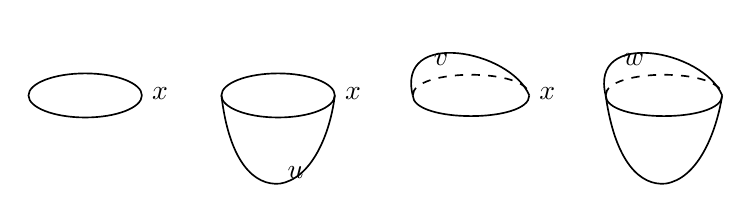
\begin{tikzpicture}[line width=0.6pt]
  \draw (0,0) ellipse (0.72 and 0.28);
  \node at (0.95,0.02) {$x$};
  \begin{scope}[shift={(2.45,0)}]
    \draw (0,0) ellipse (0.72 and 0.28);
    \draw (-0.72,0) .. controls (-0.62,-0.85) and (-0.3,-1.15) .. (0.02,-1.12)
          .. controls (0.42,-1.06) and (0.66,-0.5) .. (0.72,0);
    \node at (0.95,0.02) {$x$};
    \node at (0.22,-0.98) {$u$};
  \end{scope}
  \begin{scope}[shift={(4.9,0)}]
    \draw (-0.74,0) .. controls (-0.95,0.85) and (0.5,0.58) .. (0.74,0);
    \draw[dashed] (-0.74,0) .. controls (-0.74,0.35) and (0.74,0.35) .. (0.74,0);
    \draw (-0.74,0) .. controls (-0.74,-0.35) and (0.74,-0.35) .. (0.74,0);
    \node at (0.97,0.02) {$x$};
    \node at (-0.38,0.45) {$v$};
  \end{scope}
  \begin{scope}[shift={(7.35,0)}]
    \draw (-0.74,0) .. controls (-0.95,0.85) and (0.5,0.58) .. (0.74,0);
    \draw[dashed] (-0.74,0) .. controls (-0.74,0.35) and (0.74,0.35) .. (0.74,0);
    \draw (-0.74,0) .. controls (-0.74,-0.35) and (0.74,-0.35) .. (0.74,0);
    \draw (-0.74,0) .. controls (-0.62,-0.85) and (-0.3,-1.15) .. (0.02,-1.12)
          .. controls (0.42,-1.06) and (0.66,-0.5) .. (0.74,0);
    \node at (-0.38,0.45) {$w$};
  \end{scope}
\end{tikzpicture}
\caption{}
\label{fig:disk-gluing-sphere}
\end{figure}

\begin{example}\label{thm:action-functional-euclidean}
考虑 $W=\RR^{2n}$ 且\trSymplecticForm{}为
\[
\omega=\sum_i dp_i\wedge dq_i=d\sum_i p_i\,dq_i
\]
的情形。于是，在任何以我们的\trLoop{} $x$ 为边界的\trDisk{}上，都有
\[
\int_{D_2}u^\star\omega=\int_{S^1}x^\star(p\,dq)\text{，}
\]
从而
\[
\scr{A}_H(x)=\int_0^1\bigl(H_t\,dt-p\,dq\bigr)
\]
……即物理学家们的\emph{\trActionFunctional}。\footnote{这正是这个泛函被称作 $\scr{A}_H$ 的缘由。}
\end{example}

\begin{remark}\label{thm:asphericity-examples}
除 $\RR^{2n}$ 之外还有许多满足\cref{thm:symplectic-asphericity}的\trSymplectic\trManifold，例如诸\trTorus{} $\mathbf{T}^{2n}$、亏格至少为 $1$ 的诸曲面、诸\trCotangent{}丛（由第~14~章的\cref{ex:ch14-004-cotangent-integral}可知）。然而，无论是\trSphere{} $S^2$ 还是它的任何表亲 $\CP^n(\CC)$，都没有这个性质（这一次则靠第~14~章的\cref{ex:ch14-005-symplectic-surface}）。
\end{remark}

在我们的条件之下，$\scr{A}_H$ 确实定义了一个映射
\[
\scr{L}W\longrightarrow\RR\text{。}
\]
我们有下面的结果。

\begin{proposition}\label{thm:critical-points-periodic-orbits}
一条\trLoop{} $x$ 是 $\scr{A}_H$ 的一个\trCriticalPoint，当且仅当 $t\mapsto x(t)$ 是\trHamiltonian{}系统 $\dot{x}=X_t(x(t))$ 的一个\trPeriodic{}解。
\end{proposition}

\begin{proof}
让我们在点 $x(t)$ 处、在切向量 $Y(t)$ 上计算 $\scr{A}_H$ 的\trDifferential。我们把 $x$ 扩张成 $\tilde{x}(s,t)$，它对 $0$ 的一个邻域中的 $s$ 有定义，且使得
\[
\left\{\begin{array}{l}
\tilde{x}(0,t)=x(t)\\[2pt]
\dfrac{\partial\tilde{x}}{\partial s}(0,t)=Y(t)\text{。}
\end{array}\right.
\]
于是我们有
\[
(d\scr{A}_H)_x(Y)=\frac{\partial}{\partial s}\scr{A}_H(\tilde{x})\big|_{s=0}\text{。}
\]
让我们来研究这个导数。

\begin{figure}[htbp]
\centering
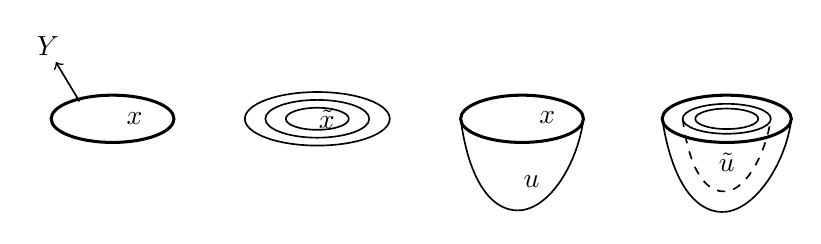
\begin{tikzpicture}[line width=0.6pt]
  \draw[line width=1.1pt] (0,0) ellipse (0.78 and 0.3);
  \draw[->] (-0.42,0.22) -- (-0.72,0.72);
  \node at (-0.82,0.92) {$Y$};
  \node at (0.28,0) {$x$};
  \begin{scope}[shift={(2.6,0)}]
    \draw (0,0) ellipse (0.92 and 0.34);
    \draw (0,0) ellipse (0.66 and 0.24);
    \draw (0,0) ellipse (0.4 and 0.14);
    \node at (0.12,0) {$\tilde{x}$};
  \end{scope}
  \begin{scope}[shift={(5.2,0)}]
    \draw[line width=1.1pt] (0,0) ellipse (0.78 and 0.3);
    \draw (-0.78,0) .. controls (-0.66,-0.9) and (-0.32,-1.2) .. (0.0,-1.16)
          .. controls (0.4,-1.1) and (0.72,-0.5) .. (0.78,0);
    \node at (0.32,0.02) {$x$};
    \node at (0.12,-0.8) {$u$};
  \end{scope}
  \begin{scope}[shift={(7.8,0)}]
    \draw[line width=1.1pt] (0,0) ellipse (0.82 and 0.3);
    \draw (-0.82,0) .. controls (-0.68,-0.9) and (-0.34,-1.22) .. (0.0,-1.18)
          .. controls (0.4,-1.12) and (0.76,-0.52) .. (0.82,0);
    \draw (0,0) ellipse (0.56 and 0.19);
    \draw (0,0) ellipse (0.4 and 0.13);
    \draw[dashed] (-0.56,0) .. controls (-0.47,-0.7) and (-0.24,-0.95) .. (0.0,-0.92)
          .. controls (0.26,-0.89) and (0.5,-0.42) .. (0.56,0);
    \node at (0.0,-0.55) {$\tilde{u}$};
  \end{scope}
\end{tikzpicture}
\caption{}
\label{fig:critical-point-computation}
\end{figure}

为此，我们选取 $u$ 的一个扩张 $\tilde{u}(s,z)$，使得
\[
\left\{\begin{array}{l}
\tilde{u}(0,z)=u(z)\\[2pt]
\tilde{u}(s,e^{2\pi it})=\tilde{x}(s,t)\text{，}
\end{array}\right.
\]
并且我们如下扩张 $Y$：令
\[
Y(z)=\frac{\partial\tilde{u}}{\partial s}(0,z)\text{。}
\]
于是
\[
\scr{A}_H(\tilde{x}(s,t))=-\int_D\tilde{u}^\star\omega+\int_0^1H_t(\tilde{x}(s,t))\,dt\text{。}
\]
对第一项求导给出
\[
\begin{aligned}
-\int_D\Bigl(\frac{d}{ds}\tilde{u}^\star\omega\Bigr)\Big|_{s=0}
&=-\int_D u^\star\bigl(\scr{L}_{Y_{(z)}}\omega\bigr)
=-\int_D u^\star\bigl(di_{Y_{(z)}}\omega\bigr)\\
&=-\int_{S^1}x^\star\bigl(i_{Y_{(t)}}\omega\bigr)
=-\int_0^1\omega\bigl(Y(t),\dot{x}(t)\bigr)\,dt\\
&=\int_0^1\omega\bigl(\dot{x}(t),Y(t)\bigr)\,dt\text{。}
\end{aligned}
\]
对第二项求导给出
\[
\begin{aligned}
\int_0^1\frac{\partial}{\partial s}H_t(\tilde{x}(s,t))\big|_{s=0}\,dt
&=\int_0^1(dH_t)_{\tilde{x}(0,t)}\bigl(Y(t)\bigr)\,dt\\
&=\int_0^1\omega_{x(t)}\bigl(Y(t),X_t(x(t))\bigr)\,dt\text{。}
\end{aligned}
\]
两者合在一起给出
\[
(d\scr{A}_H)_x(Y)=\int_0^1\omega\bigl(\dot{x}(t)-X_t(x),Y\bigr)\,dt\text{。}
\]
由此可见，\trDifferential{} $(d\scr{A}_H)_x$ 为零，当且仅当
\[
\omega\bigl(\dot{x}(t)-X_t(x),Y\bigr)=0\qquad\forall Y\text{，}
\]
也就是说，由 $\omega$ 的\trNondegenerate{}性，当且仅当 $\dot{x}=X_t(x)$，此即所要证的结果。
\end{proof}

我们将称 $x$ 是 $\scr{A}_H$ 的一个\emph{\trNondegenerate}\trCriticalPoint，如果它是一条\trNondegenerate\trTrajectory（意义见定义 5.4.4）。

\begin{remark}[\trAutonomous{}\trHamiltonian{}的情形]\label{thm:autonomous-hamiltonian-case}
\begin{enumerate}[label=(\arabic*)]
\item 我们已经看到，若 $x$ 是 $H$ 的一个\trCriticalPoint，那么常值\trTrajectory{} $x$ 就是 $\scr{A}_H$ 的一个\trCriticalPoint（其逆则对“小”的 $H$ 成立）。
\item 我们也已看到（命题 5.4.5），若 $x$ 对 $\scr{A}_H$ 而言是\trNondegenerate{}的，那么它对 $H$ 而言也是\trNondegenerate{}的（而当 $H$ “小”时其逆亦真——即注记 5.4.7）。
\item 若 $x$ 是 $\scr{A}_H$ 的一个\trCriticalPoint{}并且是一条\emph{非常值}的\trTrajectory，那么它是\trDegenerate{}的，因为向量 $X_H(x)$ 是线性映射 $T_x\varphi^1$ 的一个不动向量。\footnote{译注：原书此处作 “the field $X_H$ is a fixed point of $T_x\varphi^1$”，径把\trVectorField{}称作线性映射的“固定点”；按文意应是 $X_H$ 沿\trLoop{}取值所得的向量 $X_H(x)$ 为 $T_x\varphi^1$ 的不动向量，此处径改。——译者注}
\end{enumerate}
\end{remark}

我们的最后一条注记是：$\scr{A}_H$ 在两个相异的\trCriticalPoint{}（几何上相异，意即它们是两条几何上不同的\trTrajectory）处所取的值，可以假定是互不相同的。让我们把这个事实陈述为一条引理（后面将会用到）。

\begin{lemma}\label{thm:distinct-critical-values}
若 $x$ 与 $y$ 是 $\scr{A}_H$ 的两个几何上相异的\trCriticalPoint，则存在一个按 $\cC^2$ \trTopology{}贴近于 $H$ 的函数 $\tilde{H}$，使得 $\scr{A}_{\tilde{H}}$ 与 $\scr{A}_H$ 有相同的\trCriticalPoint{}而有不同的\trCriticalValue。\footnote{译注：这条引理按字面陈述缺少前提，并不成立：取 $H\equiv 0$，则由\cref{thm:critical-points-periodic-orbits}，一切常值\trLoop{}都是 $\scr{A}_H$ 的\trCriticalPoint{}且作用值同为 $0$，而它们两两“几何上相异”——这样的\trCriticalPoint{}有不可数多条，$\cC^2$-小的修改 $H_0$ 作为 $W$ 上的连续函数，不可能在这些\trLoop{}上取到两两不同的值（保持全部\trCriticalPoint{}亦无从谈起）。疑应把引理限定在后文实际所需的情形：$\scr{A}_H$ 的\trCriticalPoint{}只有有限多条且皆\trNondegenerate{}——此时诸 $1$-\trPeriodic\trTrajectory{}的像在时间—空间柱面 $S^1\times W$ 上互不相交，可取两两不交的\trTubularNeighborhood{}并令 $H_0$ 在其上分别取常值以分离作用值（第 9 章对\cref{thm:distinct-critical-values}的使用正是这一情形）。此处照原书排印，存疑备案。——译者注}
\end{lemma}

\begin{proof}
只需给\trHamiltonian{} $H$ 添加一个函数 $H_0$ 来做修改：这个 $H_0$ 在 $X_t$ 的 $1$-\trPeriodic\trTrajectory{}的一个邻域内为常数，按 $\cC^2$ 而言很小，并且使得对 $\scr{A}_H$ 的任意两个不同的\trCriticalPoint{} $x$ 与 $y$，都有
\[
\scr{A}_H(x)+H_0(x(0))\neq\scr{A}_H(y)+H_0(y(0))\text{。}
\]
若 $H_0$ 充分小，则 $\scr{A}_{H+H_0}$ 的\trCriticalPoint{}就是 $\scr{A}_H$ 的那些\trCriticalPoint，并且对一个\trCriticalPoint{} $x$，我们有
\[
\scr{A}_{H+H_0}(x)=\scr{A}_H(x)+\int_0^1H_0(x(t))\,dt=\scr{A}_H(x)+H_0(x(0))\text{。}
\]
\end{proof}
